\documentclass[twoside]{book}

% Packages required by doxygen
\usepackage{fixltx2e}
\usepackage{calc}
\usepackage{doxygen}
\usepackage[export]{adjustbox} % also loads graphicx
\usepackage{graphicx}
\usepackage[utf8]{inputenc}
\usepackage{makeidx}
\usepackage{multicol}
\usepackage{multirow}
\PassOptionsToPackage{warn}{textcomp}
\usepackage{textcomp}
\usepackage[nointegrals]{wasysym}
\usepackage[table]{xcolor}

% Font selection
\usepackage[T1]{fontenc}
\usepackage[scaled=.90]{helvet}
\usepackage{courier}
\usepackage{amssymb}
\usepackage{sectsty}
\renewcommand{\familydefault}{\sfdefault}
\allsectionsfont{%
  \fontseries{bc}\selectfont%
  \color{darkgray}%
}
\renewcommand{\DoxyLabelFont}{%
  \fontseries{bc}\selectfont%
  \color{darkgray}%
}
\newcommand{\+}{\discretionary{\mbox{\scriptsize$\hookleftarrow$}}{}{}}

% Page & text layout
\usepackage{geometry}
\geometry{%
  a4paper,%
  top=2.5cm,%
  bottom=2.5cm,%
  left=2.5cm,%
  right=2.5cm%
}
\tolerance=750
\hfuzz=15pt
\hbadness=750
\setlength{\emergencystretch}{15pt}
\setlength{\parindent}{0cm}
\setlength{\parskip}{3ex plus 2ex minus 2ex}
\makeatletter
\renewcommand{\paragraph}{%
  \@startsection{paragraph}{4}{0ex}{-1.0ex}{1.0ex}{%
    \normalfont\normalsize\bfseries\SS@parafont%
  }%
}
\renewcommand{\subparagraph}{%
  \@startsection{subparagraph}{5}{0ex}{-1.0ex}{1.0ex}{%
    \normalfont\normalsize\bfseries\SS@subparafont%
  }%
}
\makeatother

% Headers & footers
\usepackage{fancyhdr}
\pagestyle{fancyplain}
\fancyhead[LE]{\fancyplain{}{\bfseries\thepage}}
\fancyhead[CE]{\fancyplain{}{}}
\fancyhead[RE]{\fancyplain{}{\bfseries\leftmark}}
\fancyhead[LO]{\fancyplain{}{\bfseries\rightmark}}
\fancyhead[CO]{\fancyplain{}{}}
\fancyhead[RO]{\fancyplain{}{\bfseries\thepage}}
\fancyfoot[LE]{\fancyplain{}{}}
\fancyfoot[CE]{\fancyplain{}{}}
\fancyfoot[RE]{\fancyplain{}{\bfseries\scriptsize Generated by Doxygen }}
\fancyfoot[LO]{\fancyplain{}{\bfseries\scriptsize Generated by Doxygen }}
\fancyfoot[CO]{\fancyplain{}{}}
\fancyfoot[RO]{\fancyplain{}{}}
\renewcommand{\footrulewidth}{0.4pt}
\renewcommand{\chaptermark}[1]{%
  \markboth{#1}{}%
}
\renewcommand{\sectionmark}[1]{%
  \markright{\thesection\ #1}%
}

% Indices & bibliography
\usepackage{natbib}
\usepackage[titles]{tocloft}
\setcounter{tocdepth}{3}
\setcounter{secnumdepth}{5}
\makeindex

% Hyperlinks (required, but should be loaded last)
\usepackage{ifpdf}
\ifpdf
  \usepackage[pdftex,pagebackref=true]{hyperref}
\else
  \usepackage[ps2pdf,pagebackref=true]{hyperref}
\fi
\hypersetup{%
  colorlinks=true,%
  linkcolor=blue,%
  citecolor=blue,%
  unicode%
}

% Custom commands
\newcommand{\clearemptydoublepage}{%
  \newpage{\pagestyle{empty}\cleardoublepage}%
}

\usepackage{caption}
\captionsetup{labelsep=space,justification=centering,font={bf},singlelinecheck=off,skip=4pt,position=top}

%===== C O N T E N T S =====

\begin{document}

% Titlepage & ToC
\hypersetup{pageanchor=false,
             bookmarksnumbered=true,
             pdfencoding=unicode
            }
\pagenumbering{roman}
\begin{titlepage}
\vspace*{7cm}
\begin{center}%
{\Large My Project }\\
\vspace*{1cm}
{\large Generated by Doxygen 1.8.11}\\
\end{center}
\end{titlepage}
\clearemptydoublepage
\tableofcontents
\clearemptydoublepage
\pagenumbering{arabic}
\hypersetup{pageanchor=true}

%--- Begin generated contents ---
\chapter{File Index}
\section{File List}
Here is a list of all documented files with brief descriptions\+:\begin{DoxyCompactList}
\item\contentsline{section}{\hyperlink{fumadores_8cpp}{fumadores.\+cpp} \\*Simula a un estanquero y sus fumadores }{\pageref{fumadores_8cpp}}{}
\item\contentsline{section}{\hyperlink{productor__consumidor_8cpp}{productor\+\_\+consumidor.\+cpp} \\*Simula la produccion y consumicion sincronizada de datos en un buffer }{\pageref{productor__consumidor_8cpp}}{}
\end{DoxyCompactList}

\chapter{File Documentation}
\hypertarget{fumadores_8cpp}{}\section{fumadores.\+cpp File Reference}
\label{fumadores_8cpp}\index{fumadores.\+cpp@{fumadores.\+cpp}}


Simula a un estanquero y sus fumadores.  


{\ttfamily \#include $<$iostream$>$}\\*
{\ttfamily \#include $<$cassert$>$}\\*
{\ttfamily \#include $<$pthread.\+h$>$}\\*
{\ttfamily \#include $<$semaphore.\+h$>$}\\*
{\ttfamily \#include $<$unistd.\+h$>$}\\*
{\ttfamily \#include $<$stdlib.\+h$>$}\\*
{\ttfamily \#include $<$time.\+h$>$}\\*
Include dependency graph for fumadores.\+cpp\+:
\nopagebreak
\begin{figure}[H]
\begin{center}
\leavevmode
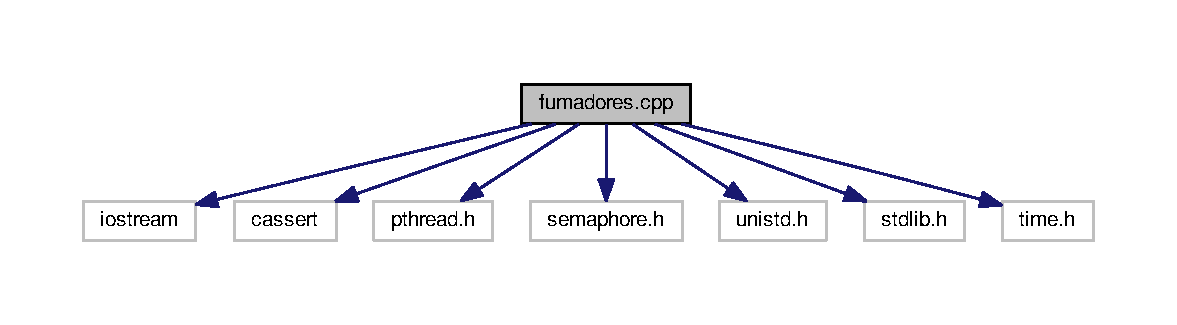
\includegraphics[width=350pt]{fumadores_8cpp__incl}
\end{center}
\end{figure}
\subsection*{Functions}
\begin{DoxyCompactItemize}
\item 
void \hyperlink{fumadores_8cpp_a77acc9846657a4b03ecfcea2a4ce1040}{retraso\+\_\+aleatorio} (const float smin, const float smax)
\begin{DoxyCompactList}\small\item\em introduce un retraso aleatorio de duración comprendida entre \textquotesingle{}smin\textquotesingle{} y \textquotesingle{}smax\textquotesingle{} (dados en segundos) \end{DoxyCompactList}\item 
void \hyperlink{fumadores_8cpp_aae7f7f70c42d51e3633a7fd8131d5654}{fumar} (int num\+\_\+fum)
\begin{DoxyCompactList}\small\item\em Función que simula la accion de fumar. Mostrara por pantalla el fumador que esta fumando. \end{DoxyCompactList}\item 
void $\ast$ \hyperlink{fumadores_8cpp_a4cb283a6b00c04d6024c8778816665ff}{funcion\+\_\+estanquero} (void $\ast$)
\begin{DoxyCompactList}\small\item\em Función que ejecuta la hebra del estanquero. \end{DoxyCompactList}\item 
void $\ast$ \hyperlink{fumadores_8cpp_ad354d1e6fb952c6892327b6077eeb235}{funcion\+\_\+fumador} (void $\ast$num\+\_\+fum\+\_\+void)
\begin{DoxyCompactList}\small\item\em Función que ejecuta la hebra del fumador. \end{DoxyCompactList}\item 
int {\bfseries main} ()\hypertarget{fumadores_8cpp_ae66f6b31b5ad750f1fe042a706a4e3d4}{}\label{fumadores_8cpp_ae66f6b31b5ad750f1fe042a706a4e3d4}

\end{DoxyCompactItemize}
\subsection*{Variables}
\begin{DoxyCompactItemize}
\item 
sem\+\_\+t \hyperlink{fumadores_8cpp_a297407bf441f68b65a7f88bb36341cb0}{fumadores} \mbox{[}3\mbox{]}\hypertarget{fumadores_8cpp_a297407bf441f68b65a7f88bb36341cb0}{}\label{fumadores_8cpp_a297407bf441f68b65a7f88bb36341cb0}

\begin{DoxyCompactList}\small\item\em Declaramos los semaforos tipo $<$sem\+\_\+t$>$ para cada uno de los actores del problema. \end{DoxyCompactList}\item 
sem\+\_\+t {\bfseries estanquero}\hypertarget{fumadores_8cpp_ae12c884620a9ee83c89b98d8253dcaf9}{}\label{fumadores_8cpp_ae12c884620a9ee83c89b98d8253dcaf9}

\item 
sem\+\_\+t {\bfseries mutex}\hypertarget{fumadores_8cpp_a69dc6cbabd0ff91786e988284cd51c39}{}\label{fumadores_8cpp_a69dc6cbabd0ff91786e988284cd51c39}

\end{DoxyCompactItemize}


\subsection{Detailed Description}
Simula a un estanquero y sus fumadores. 

\begin{DoxyAuthor}{Author}
Angel Barrilao 
\end{DoxyAuthor}


\subsection{Function Documentation}
\index{fumadores.\+cpp@{fumadores.\+cpp}!fumar@{fumar}}
\index{fumar@{fumar}!fumadores.\+cpp@{fumadores.\+cpp}}
\subsubsection[{\texorpdfstring{fumar(int num\+\_\+fum)}{fumar(int num_fum)}}]{\setlength{\rightskip}{0pt plus 5cm}void fumar (
\begin{DoxyParamCaption}
\item[{int}]{num\+\_\+fum}
\end{DoxyParamCaption}
)}\hypertarget{fumadores_8cpp_aae7f7f70c42d51e3633a7fd8131d5654}{}\label{fumadores_8cpp_aae7f7f70c42d51e3633a7fd8131d5654}


Función que simula la accion de fumar. Mostrara por pantalla el fumador que esta fumando. 


\begin{DoxyParams}{Parameters}
{\em Recibe} & el id de un fumador como entero \\
\hline
\end{DoxyParams}
\index{fumadores.\+cpp@{fumadores.\+cpp}!funcion\+\_\+estanquero@{funcion\+\_\+estanquero}}
\index{funcion\+\_\+estanquero@{funcion\+\_\+estanquero}!fumadores.\+cpp@{fumadores.\+cpp}}
\subsubsection[{\texorpdfstring{funcion\+\_\+estanquero(void $\ast$)}{funcion_estanquero(void *)}}]{\setlength{\rightskip}{0pt plus 5cm}void$\ast$ funcion\+\_\+estanquero (
\begin{DoxyParamCaption}
\item[{void $\ast$}]{}
\end{DoxyParamCaption}
)}\hypertarget{fumadores_8cpp_a4cb283a6b00c04d6024c8778816665ff}{}\label{fumadores_8cpp_a4cb283a6b00c04d6024c8778816665ff}


Función que ejecuta la hebra del estanquero. 


\begin{DoxyParams}{Parameters}
{\em ptr} & tipo void \\
\hline
\end{DoxyParams}
\index{fumadores.\+cpp@{fumadores.\+cpp}!funcion\+\_\+fumador@{funcion\+\_\+fumador}}
\index{funcion\+\_\+fumador@{funcion\+\_\+fumador}!fumadores.\+cpp@{fumadores.\+cpp}}
\subsubsection[{\texorpdfstring{funcion\+\_\+fumador(void $\ast$num\+\_\+fum\+\_\+void)}{funcion_fumador(void *num_fum_void)}}]{\setlength{\rightskip}{0pt plus 5cm}void$\ast$ funcion\+\_\+fumador (
\begin{DoxyParamCaption}
\item[{void $\ast$}]{num\+\_\+fum\+\_\+void}
\end{DoxyParamCaption}
)}\hypertarget{fumadores_8cpp_ad354d1e6fb952c6892327b6077eeb235}{}\label{fumadores_8cpp_ad354d1e6fb952c6892327b6077eeb235}


Función que ejecuta la hebra del fumador. 


\begin{DoxyParams}{Parameters}
{\em ptr} & tipo void, indica el ID del fumador \\
\hline
\end{DoxyParams}
\index{fumadores.\+cpp@{fumadores.\+cpp}!retraso\+\_\+aleatorio@{retraso\+\_\+aleatorio}}
\index{retraso\+\_\+aleatorio@{retraso\+\_\+aleatorio}!fumadores.\+cpp@{fumadores.\+cpp}}
\subsubsection[{\texorpdfstring{retraso\+\_\+aleatorio(const float smin, const float smax)}{retraso_aleatorio(const float smin, const float smax)}}]{\setlength{\rightskip}{0pt plus 5cm}void retraso\+\_\+aleatorio (
\begin{DoxyParamCaption}
\item[{const float}]{smin, }
\item[{const float}]{smax}
\end{DoxyParamCaption}
)}\hypertarget{fumadores_8cpp_a77acc9846657a4b03ecfcea2a4ce1040}{}\label{fumadores_8cpp_a77acc9846657a4b03ecfcea2a4ce1040}


introduce un retraso aleatorio de duración comprendida entre \textquotesingle{}smin\textquotesingle{} y \textquotesingle{}smax\textquotesingle{} (dados en segundos) 


\begin{DoxyParams}{Parameters}
{\em smin} & minimo de segundos \\
\hline
{\em smax} & maximo de segundos \\
\hline
\end{DoxyParams}

\hypertarget{productor__consumidor_8cpp}{}\section{productor\+\_\+consumidor.\+cpp File Reference}
\label{productor__consumidor_8cpp}\index{productor\+\_\+consumidor.\+cpp@{productor\+\_\+consumidor.\+cpp}}


Simula la produccion y consumicion sincronizada de datos en un buffer.  


{\ttfamily \#include $<$iostream$>$}\\*
{\ttfamily \#include $<$cassert$>$}\\*
{\ttfamily \#include $<$pthread.\+h$>$}\\*
{\ttfamily \#include $<$semaphore.\+h$>$}\\*
{\ttfamily \#include $<$unistd.\+h$>$}\\*
{\ttfamily \#include $<$stdlib.\+h$>$}\\*
{\ttfamily \#include $<$time.\+h$>$}\\*
Include dependency graph for productor\+\_\+consumidor.\+cpp\+:
\nopagebreak
\begin{figure}[H]
\begin{center}
\leavevmode
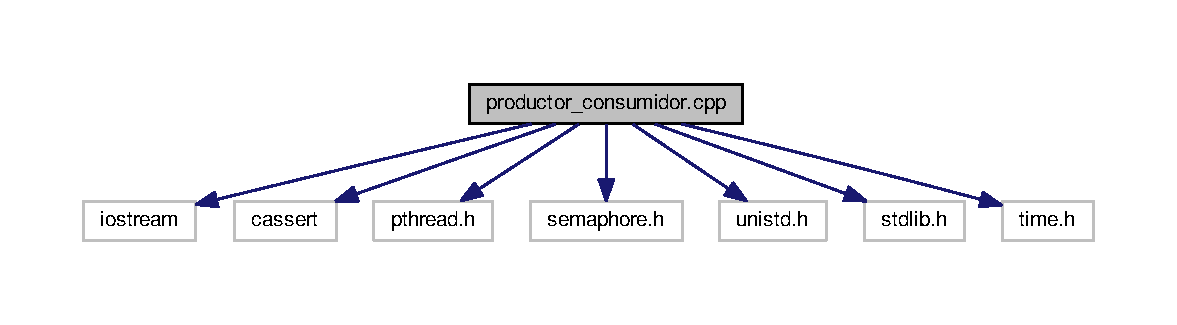
\includegraphics[width=350pt]{productor__consumidor_8cpp__incl}
\end{center}
\end{figure}
\subsection*{Functions}
\begin{DoxyCompactItemize}
\item 
vector$<$ int $>$ {\bfseries buffer} (tam\+\_\+vector)\hypertarget{productor__consumidor_8cpp_a964e7e09b4b6895d628d696eacb59586}{}\label{productor__consumidor_8cpp_a964e7e09b4b6895d628d696eacb59586}

\item 
void \hyperlink{productor__consumidor_8cpp_a77acc9846657a4b03ecfcea2a4ce1040}{retraso\+\_\+aleatorio} (const float smin, const float smax)
\begin{DoxyCompactList}\small\item\em introduce un retraso aleatorio de duración comprendida entre \textquotesingle{}smin\textquotesingle{} y \textquotesingle{}smax\textquotesingle{} (dados en segundos) \end{DoxyCompactList}\item 
unsigned \hyperlink{productor__consumidor_8cpp_a4c8153f26984dcad96b65a31c0888a53}{producir\+\_\+dato} ()
\begin{DoxyCompactList}\small\item\em Función que simula la producción de un dato. \end{DoxyCompactList}\item 
void \hyperlink{productor__consumidor_8cpp_ad4a4be632dec3a2b3a0ae99b2bc278e4}{consumir\+\_\+dato} (int dato)
\begin{DoxyCompactList}\small\item\em Función que simula la consumicion de un dato. \end{DoxyCompactList}\item 
void $\ast$ \hyperlink{productor__consumidor_8cpp_acac6e9cb1cf8e642adf05f75d12e8d07}{funcion\+\_\+productor} (void $\ast$)
\begin{DoxyCompactList}\small\item\em Función que ejecuta la hebra del productor. \end{DoxyCompactList}\item 
void $\ast$ \hyperlink{productor__consumidor_8cpp_af24194dc7d3d27155cd9803cbc4186c1}{funcion\+\_\+consumidor} (void $\ast$)
\begin{DoxyCompactList}\small\item\em Función que ejecuta la hebra del consumidor. \end{DoxyCompactList}\item 
int {\bfseries main} ()\hypertarget{productor__consumidor_8cpp_ae66f6b31b5ad750f1fe042a706a4e3d4}{}\label{productor__consumidor_8cpp_ae66f6b31b5ad750f1fe042a706a4e3d4}

\end{DoxyCompactItemize}
\subsection*{Variables}
\begin{DoxyCompactItemize}
\item 
const unsigned \hyperlink{productor__consumidor_8cpp_a973b122746d5543e92200f47639b0181}{num\+\_\+items} = 40\hypertarget{productor__consumidor_8cpp_a973b122746d5543e92200f47639b0181}{}\label{productor__consumidor_8cpp_a973b122746d5543e92200f47639b0181}

\begin{DoxyCompactList}\small\item\em Declaramos las variables tipo $<$const unsigned$>$=\char`\"{}\char`\"{}$>$ para num\+\_\+items y tam\+\_\+vector. Declaramos los semaforos , un buffer de tipo $<$vector$>$ y una varible de tipo $<$int$>$ para la ocupacion del buffer. \end{DoxyCompactList}\item 
const unsigned {\bfseries tam\+\_\+vector} = 10\hypertarget{productor__consumidor_8cpp_abfd2cdfb8b14ae607f76cae4cbd0f32d}{}\label{productor__consumidor_8cpp_abfd2cdfb8b14ae607f76cae4cbd0f32d}

\item 
sem\+\_\+t {\bfseries producir}\hypertarget{productor__consumidor_8cpp_a6d1cdf6834984f21984c27cfc3ae0593}{}\label{productor__consumidor_8cpp_a6d1cdf6834984f21984c27cfc3ae0593}

\item 
sem\+\_\+t {\bfseries consumir}\hypertarget{productor__consumidor_8cpp_a7caf70564028f5de02be1161e9e108ea}{}\label{productor__consumidor_8cpp_a7caf70564028f5de02be1161e9e108ea}

\item 
sem\+\_\+t {\bfseries mutex}\hypertarget{productor__consumidor_8cpp_a69dc6cbabd0ff91786e988284cd51c39}{}\label{productor__consumidor_8cpp_a69dc6cbabd0ff91786e988284cd51c39}

\item 
int {\bfseries ocupacion} =0\hypertarget{productor__consumidor_8cpp_ae0decea53915c967f1d213f3fe075b6b}{}\label{productor__consumidor_8cpp_ae0decea53915c967f1d213f3fe075b6b}

\end{DoxyCompactItemize}


\subsection{Detailed Description}
Simula la produccion y consumicion sincronizada de datos en un buffer. 

\begin{DoxyAuthor}{Author}
Angel Barrilao 
\end{DoxyAuthor}


\subsection{Function Documentation}
\index{productor\+\_\+consumidor.\+cpp@{productor\+\_\+consumidor.\+cpp}!consumir\+\_\+dato@{consumir\+\_\+dato}}
\index{consumir\+\_\+dato@{consumir\+\_\+dato}!productor\+\_\+consumidor.\+cpp@{productor\+\_\+consumidor.\+cpp}}
\subsubsection[{\texorpdfstring{consumir\+\_\+dato(int dato)}{consumir_dato(int dato)}}]{\setlength{\rightskip}{0pt plus 5cm}void consumir\+\_\+dato (
\begin{DoxyParamCaption}
\item[{int}]{dato}
\end{DoxyParamCaption}
)}\hypertarget{productor__consumidor_8cpp_ad4a4be632dec3a2b3a0ae99b2bc278e4}{}\label{productor__consumidor_8cpp_ad4a4be632dec3a2b3a0ae99b2bc278e4}


Función que simula la consumicion de un dato. 


\begin{DoxyParams}{Parameters}
{\em dato} & Paramero de entrada que se mostrara en pantalla \\
\hline
\end{DoxyParams}
\index{productor\+\_\+consumidor.\+cpp@{productor\+\_\+consumidor.\+cpp}!funcion\+\_\+consumidor@{funcion\+\_\+consumidor}}
\index{funcion\+\_\+consumidor@{funcion\+\_\+consumidor}!productor\+\_\+consumidor.\+cpp@{productor\+\_\+consumidor.\+cpp}}
\subsubsection[{\texorpdfstring{funcion\+\_\+consumidor(void $\ast$)}{funcion_consumidor(void *)}}]{\setlength{\rightskip}{0pt plus 5cm}void$\ast$ funcion\+\_\+consumidor (
\begin{DoxyParamCaption}
\item[{void $\ast$}]{}
\end{DoxyParamCaption}
)}\hypertarget{productor__consumidor_8cpp_af24194dc7d3d27155cd9803cbc4186c1}{}\label{productor__consumidor_8cpp_af24194dc7d3d27155cd9803cbc4186c1}


Función que ejecuta la hebra del consumidor. 

\begin{DoxyReturn}{Returns}
N\+U\+LL 
\end{DoxyReturn}

\begin{DoxyParams}{Parameters}
{\em ptr} & tipo void \\
\hline
\end{DoxyParams}
\index{productor\+\_\+consumidor.\+cpp@{productor\+\_\+consumidor.\+cpp}!funcion\+\_\+productor@{funcion\+\_\+productor}}
\index{funcion\+\_\+productor@{funcion\+\_\+productor}!productor\+\_\+consumidor.\+cpp@{productor\+\_\+consumidor.\+cpp}}
\subsubsection[{\texorpdfstring{funcion\+\_\+productor(void $\ast$)}{funcion_productor(void *)}}]{\setlength{\rightskip}{0pt plus 5cm}void$\ast$ funcion\+\_\+productor (
\begin{DoxyParamCaption}
\item[{void $\ast$}]{}
\end{DoxyParamCaption}
)}\hypertarget{productor__consumidor_8cpp_acac6e9cb1cf8e642adf05f75d12e8d07}{}\label{productor__consumidor_8cpp_acac6e9cb1cf8e642adf05f75d12e8d07}


Función que ejecuta la hebra del productor. 

\begin{DoxyReturn}{Returns}
N\+U\+LL 
\end{DoxyReturn}

\begin{DoxyParams}{Parameters}
{\em ptr} & tipo void \\
\hline
\end{DoxyParams}
\index{productor\+\_\+consumidor.\+cpp@{productor\+\_\+consumidor.\+cpp}!producir\+\_\+dato@{producir\+\_\+dato}}
\index{producir\+\_\+dato@{producir\+\_\+dato}!productor\+\_\+consumidor.\+cpp@{productor\+\_\+consumidor.\+cpp}}
\subsubsection[{\texorpdfstring{producir\+\_\+dato()}{producir_dato()}}]{\setlength{\rightskip}{0pt plus 5cm}unsigned producir\+\_\+dato (
\begin{DoxyParamCaption}
{}
\end{DoxyParamCaption}
)}\hypertarget{productor__consumidor_8cpp_a4c8153f26984dcad96b65a31c0888a53}{}\label{productor__consumidor_8cpp_a4c8153f26984dcad96b65a31c0888a53}


Función que simula la producción de un dato. 

\begin{DoxyReturn}{Returns}
Devuelve una cifra 
\end{DoxyReturn}

\begin{DoxyRetVals}{Return values}
{\em unsigned} & \\
\hline
\end{DoxyRetVals}
\index{productor\+\_\+consumidor.\+cpp@{productor\+\_\+consumidor.\+cpp}!retraso\+\_\+aleatorio@{retraso\+\_\+aleatorio}}
\index{retraso\+\_\+aleatorio@{retraso\+\_\+aleatorio}!productor\+\_\+consumidor.\+cpp@{productor\+\_\+consumidor.\+cpp}}
\subsubsection[{\texorpdfstring{retraso\+\_\+aleatorio(const float smin, const float smax)}{retraso_aleatorio(const float smin, const float smax)}}]{\setlength{\rightskip}{0pt plus 5cm}void retraso\+\_\+aleatorio (
\begin{DoxyParamCaption}
\item[{const float}]{smin, }
\item[{const float}]{smax}
\end{DoxyParamCaption}
)}\hypertarget{productor__consumidor_8cpp_a77acc9846657a4b03ecfcea2a4ce1040}{}\label{productor__consumidor_8cpp_a77acc9846657a4b03ecfcea2a4ce1040}


introduce un retraso aleatorio de duración comprendida entre \textquotesingle{}smin\textquotesingle{} y \textquotesingle{}smax\textquotesingle{} (dados en segundos) 


\begin{DoxyParams}{Parameters}
{\em smin} & minimo de segundos \\
\hline
{\em smax} & maximo de segundos \\
\hline
\end{DoxyParams}

%--- End generated contents ---

% Index
\backmatter
\newpage
\phantomsection
\clearemptydoublepage
\addcontentsline{toc}{chapter}{Index}
\printindex

\end{document}
